\begin{figure}[p]
\centering
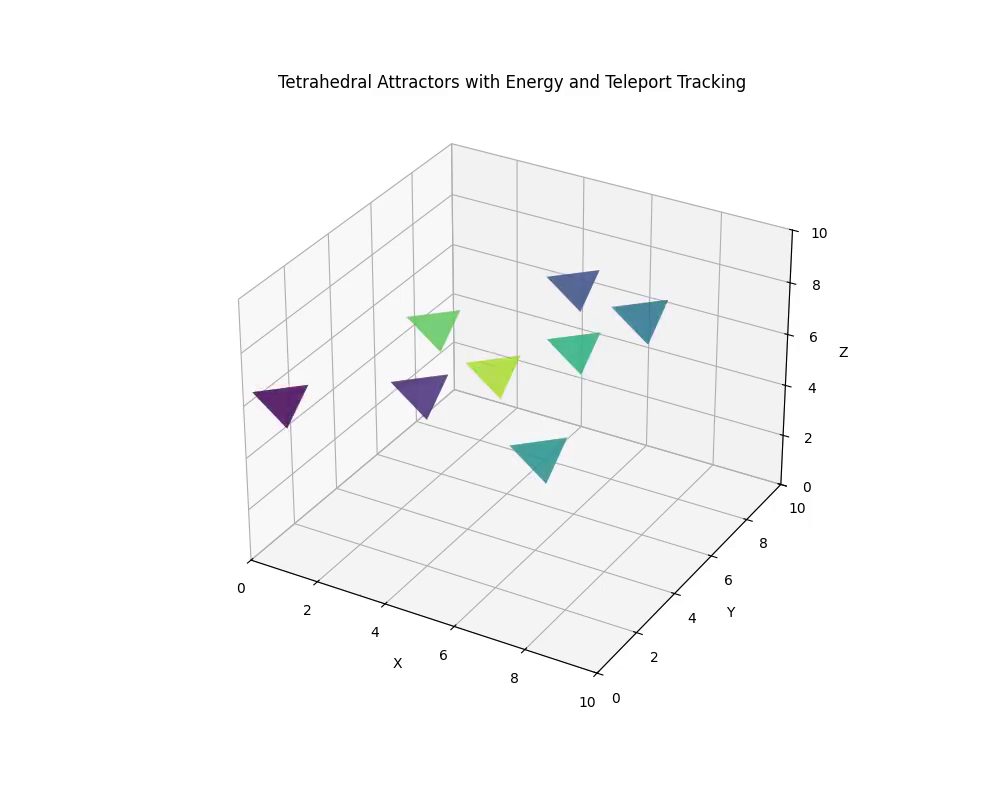
\includegraphics[width=0.485\linewidth,height=0.32\textheight,keepaspectratio]{figures/F16_0.png}
\hfill
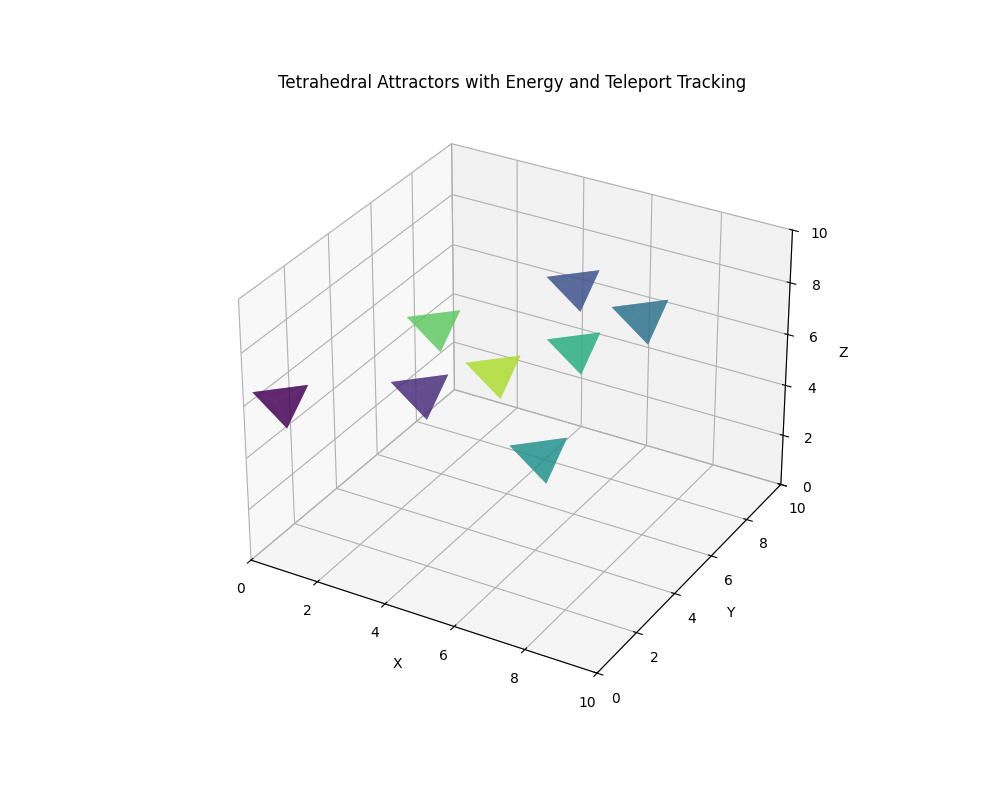
\includegraphics[width=0.485\linewidth,height=0.32\textheight,keepaspectratio]{figures/F16_1.png}
\par\medskip
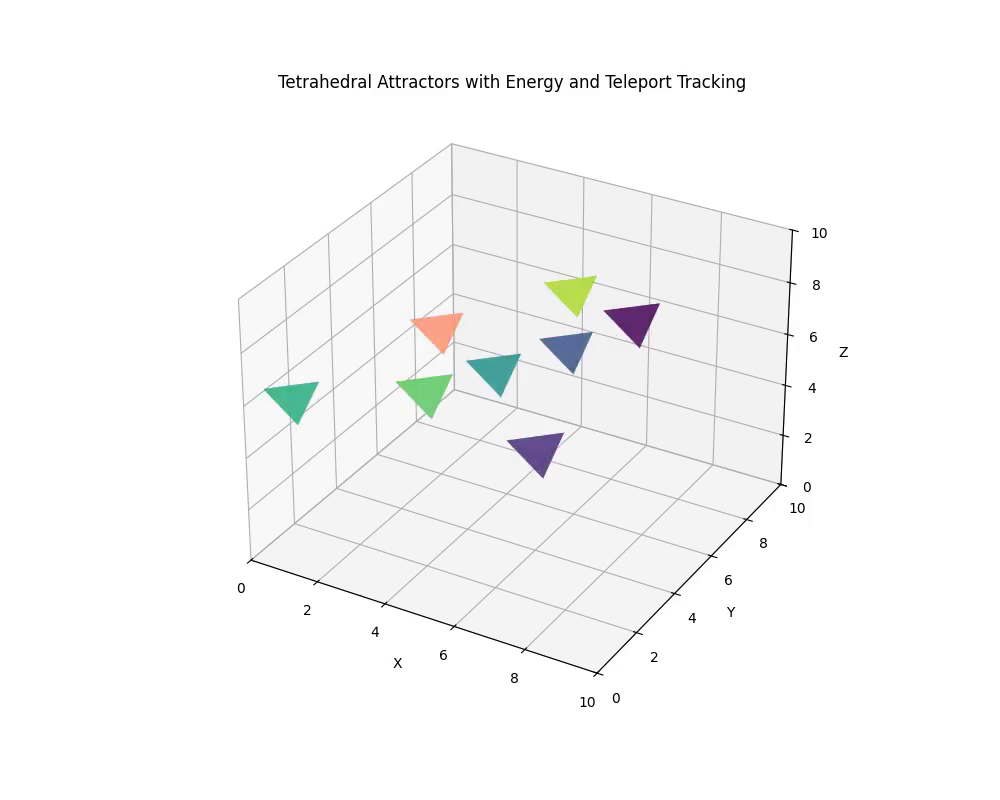
\includegraphics[width=0.485\linewidth,height=0.32\textheight,keepaspectratio]{figures/F16_2.png}
\hfill
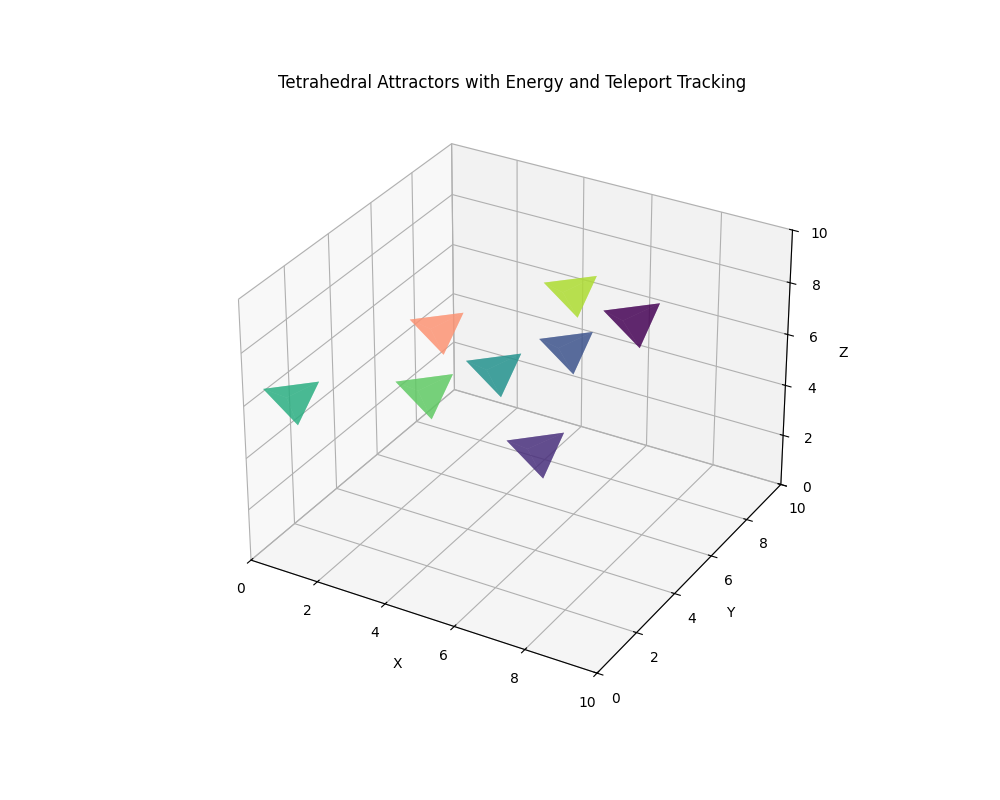
\includegraphics[width=0.485\linewidth,height=0.32\textheight,keepaspectratio]{figures/F16_3.png}
\par\medskip
\caption[Two sampled movie-to-record correspondences]{ORIGINAL movie content at left; DERIVED renderings of ORIGINAL saved B states at right. Top: movie frame 1 versus Bq2. Bottom: movie frame 6 versus Bq7. These are two of the eight fixed comparisons already performed in Study 03 using source geometry and current rendering defaults. No trajectories or fitted parameters were generated. Strong content agreement supports a candidate correspondence, while the original-run join remains formally UNLINKED. \cite{study03}}
\label{fig:F16}
\end{figure}
